\documentclass{article}
\usepackage{amsmath}
\usepackage{moreverb}
\usepackage{amssymb}
\usepackage{graphicx}
\usepackage{mathtools}
\usepackage{tikz}
\usepackage{pgfplots}
\usetikzlibrary{arrows,shapes, positioning}
\DeclarePairedDelimiter\floor{\lfloor}{\rfloor}
\let\biconditional\leftrightarrow
\addtolength{\oddsidemargin}{-.875in}
\addtolength{\evensidemargin}{-.875in}
\addtolength{\textwidth}{1.75in}
\addtolength{\topmargin}{-.875in}
\addtolength{\textheight}{1.75in}
\newenvironment{customlegend}[1][]{%
    \begingroup
    % inits/clears the lists (which might be populated from previous
    % axes):
    \csname pgfplots@init@cleared@structures\endcsname
    \pgfplotsset{#1}%
}{%
    % draws the legend:
    \csname pgfplots@createlegend\endcsname
    \endgroup
}%

% makes \addlegendimage available (typically only available within an
% axis environment):
\def\addlegendimage{\csname pgfplots@addlegendimage\endcsname}

\pgfkeys{/pgfplots/number in legend/.style={%
        /pgfplots/legend image code/.code={%
            \node at (0.295,-0.0225){#1};
        },%
    },
}

\begin{document}
\title{\textbf{Comp 512: Deliverable 1}}
\author{Jacob Erringtom (260636023)  \\ Alexandre Laporte (260635979)}
\date{October 6th, 2015}
\maketitle
\begin{description}
\item[Part 1: WebServices]\hfill
	\begin{description}
		\item[General Architecture:]\hfill\\	
			The design of the webservies component of the deliverable was centered around creating a the middleware manager. In order
			to acheive this we created a middleware server which implements the server's Resource Manager interface.\\
			This middleware program is implemented as follows, it manages three Resource Managers which each point to servers, namely the flight Manager, 
			car Manager and room Manager. Its task is then to process requests from a client and forward these to the appropriate server for handling, returning
			value provided by the server back to the client. \\
			A notable exception to this general process is the handling of adding clients which is handled by the middleware in conjunction with the database server (see below).\\ \\ 
			The server code also had to be changed in order to account for concurrent access to data and synchronization between servers. To this end we added an additional server, our database,
			which hosts a POSTGRESQL database. All the server code was then changed to rather than use distributed hash tables, query and write to the database. This gives us a guarantee that
			upon concurrent access of data no problems arize. Additionally connections to the database are handled using DBCP connection pools ensuring that concurrent connections are handled without issue.  \\
			Additionally in the case of customer queries from the client the middleware interfaces directly with the database, likewise with the reserveItinerary function. \\
			This means that our system has the following structure:
			\item
			\begin{equation}
			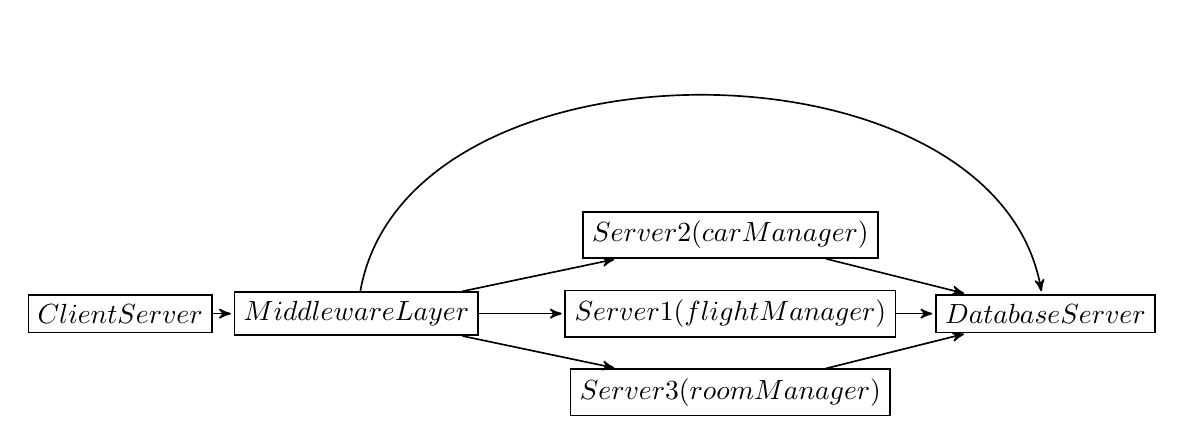
\begin{tikzpicture}[->,>=stealth',shorten >=1pt,auto,node distance=1cm,semithick]
			\node[draw] (rect)        			(A) 				{$Client Server$};
			\node[draw] (rect)	       			(B) [right of=A,xshift=2cm] {$Middleware Layer$};
			\node[draw] (rect)        (C) [right of=B,xshift=3.75cm] {$Server 1(flight Manager)$};
			\node[draw] (rect) (D)[above of=C] {$Server 2(car Manager)$}; 
			\node[draw] (rect) 	  (E)[below of=C] {$Server 3(room Manager)$};
			\node[draw] (rect)	  (F)[right of = C, xshift=3cm]{$Database Server$}; 
			

			\path 
			(A) edge              node{}  (B)
			(B) edge 			  node {} (C)
				edge			  node {} (D)
				edge			  node {} (E)
				edge[out=80,in=100]  node {} (F)
			(C) edge 			  node {}(F)
			(D) edge		 	  node {}(F)
			(E) edge 			  node {} (F); 
			\end{tikzpicture}
			\end{equation}
			\clearpage
		\item[Database Architecture:]
			 For clarity the database architecture is included here 
	\end{description}
			\begin{equation}
			 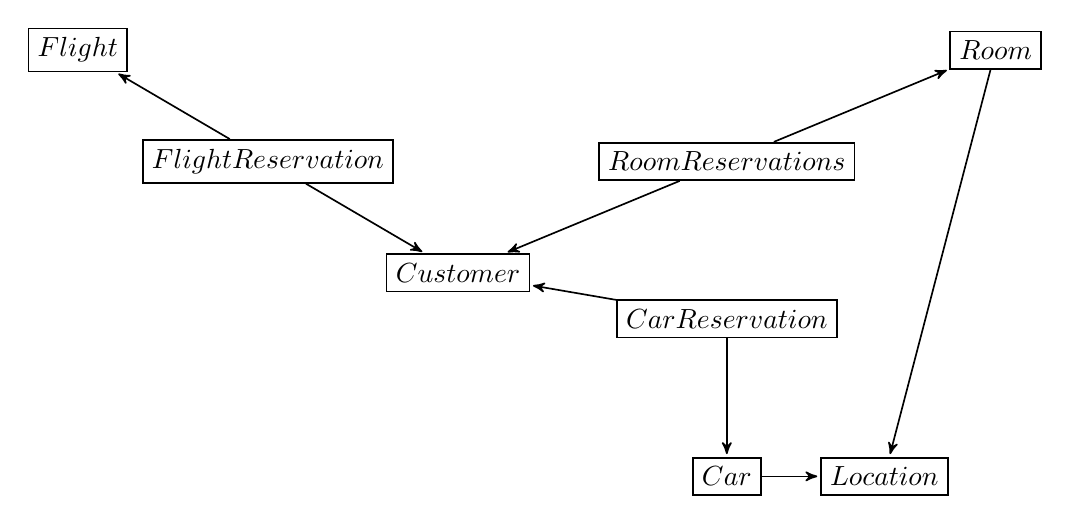
\begin{tikzpicture}[->,>=stealth',shorten >=1pt,auto,node distance=2cm,semithick]
			 \node[draw] (rect)		(A) {$Flight$};
			 \node[draw] (rect)		(B) [below right of=A,xshift=1cm] {$FlightReservation$};
			 \node[draw] (rect)		(C) [below right of=B,xshift=1cm] {$Customer$};
			 \node[draw] (rect)		(D) [above right of=C,xshift=2cm] {$RoomReservations$};
			 \node[draw] (rect) 	(E) [below of=D] {$CarReservation$};
			 \node[draw] (rect)		(F) [below of=E] {$Car$};
			 \node[draw] (rect)		(G) [right of=F] {$Location$}; 
			 \node[draw] (rect)		(H) [above right of=D, xshift=2cm]{$Room$}; 
			 \path
			 (A)
			 (B) edge node{} (A)
			 	edge  node{}  (C)
			 (C)
			 (D) edge node{} (C)
			 	 edge node{} (H)
			 (E) edge node{} (C)
			  	 edge node{} (F)
			 (F) edge node{} (G)
			 (G)
			 (H) edge node{} (G); 
 			 \end{tikzpicture}
 			 \end{equation}
 \item[Part 2: Socket Code] \hfill \\ 
 	The overaching architecture of the websockets code is identical to the structure shown in (1). As such the description will be focused on the
 	implementations of webservices on top of websockets. \\
 	We begin by creating an executor service and oppening a websocket. The server then listens on the socket of all incomming connections, once a connection is opened it is accpted and
 	packaged into a request context which contains a RequestManager and the socket connection. The request manager implements runnable and is passed to the executor service which assigns the connection a thread and invokes Request Manager's run. The executor service guarantees that connections are run asynchronously and act as a threadpool. \\
 	The RequestManager's run fetches the socket from the request context, upon receiving an input stream we use Java builtin serialization to pass our own request and response objects,
 	this allows us to gracefully handle exceptions in a network transparent manner. The Resquest Handler of the recipient then uses Java's build in reflection toolset to identify which method should be invoked providing us with a method of remote method invocation through sockets. As per the webservices code database access is handled through DBCP connection pools. 
 	
  	\begin{equation}
  	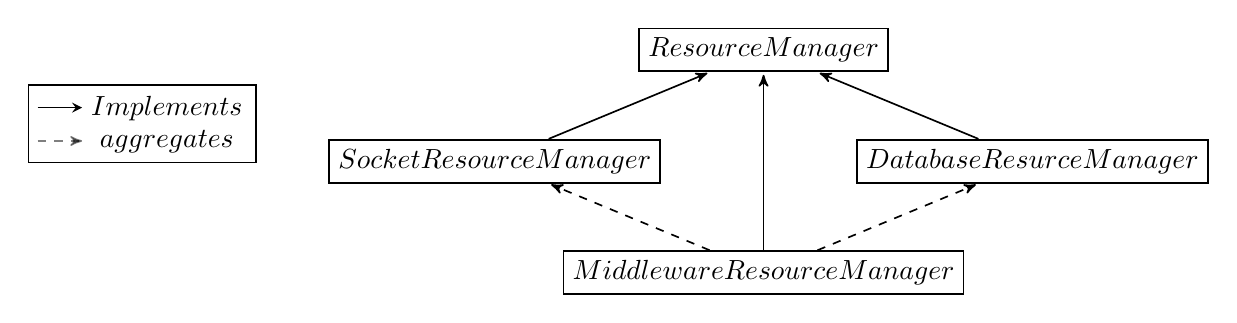
\begin{tikzpicture}[->,>=stealth',shorten >=1pt,auto,node distance=2cm,semithick]
 	 	\node[draw] (rect) (A)[xshift=4cm] {$SocketResourceManager$};
 	 	\node[draw] (rect) (B) [above right of=A,xshift=2cm] {$ResourceManager$};
 	 	\node[draw] (rect) (C) [below right of=B, xshift=2cm]{$DatabaseResurceManager$};
 	 	\node[draw] (rect) (D) [below right of=A, xshift=2cm]{$MiddlewareResourceManager$}; 
 	 	\path
 	 	(A) edge node{} (B)
 	 	(B)
 	 	(C) edge node{} (B)
 	 	(D) edge node{} (B)
 	 		edge[dashed] node{} (C)
 	 		edge[dashed] node{} (A);
 	 	\begin{customlegend}[
			legend entries={ % <= in the following there are the entries
			$Implements$,
			$aggregates$
			}] % <= to define position and font legend
			% the following are the "images" and numbers in the legend
			\addlegendimage{-stealth,black,opacity=1}
			\addlegendimage{black,dashed,opacity=0.5}
			\end{customlegend} 
  	 \end{tikzpicture}
  	 \end{equation}
  	 The above diagram can be read as follows, SocketResourceManagers represent client Resource managers, their purpose being to communicate with the middleware 
  	 and forward method calls. The databaseResourceManager represents the server Resource managers where every call is either a database read or write operation. 
  	 The MiddlewareResourceManager aggregates both these managers as the middleware can either act as a client to the databaseResourceManager or perform database operations,
  	 specifically in the event of customer operations.  
  	\end{description}
\end{document}